\documentclass[runningheads]{llncs}
\usepackage{lmodern}
\usepackage[T1]{fontenc}
\usepackage{microtype}
\usepackage{amsmath,amssymb}
\usepackage{graphicx}
\usepackage{booktabs}
\usepackage{url}
\usepackage{tikz}
\usetikzlibrary{arrows.meta,positioning,calc,fit,shapes.geometric,backgrounds}
\usepackage{listings}
\usepackage{multirow}
\usepackage{colortbl}
\usepackage{enumitem}
\setlist{noitemsep,topsep=1pt,parsep=0pt,partopsep=0pt}
\setlength{\parskip}{0pt}
\raggedbottom
\setlength{\textfloatsep}{7pt plus 2pt minus 2pt}
\setlength{\floatsep}{7pt plus 2pt minus 2pt}
\setlength{\intextsep}{7pt plus 2pt minus 2pt}
\setlength{\abovecaptionskip}{4pt}
\setlength{\belowcaptionskip}{4pt}
\lstset{basicstyle=\ttfamily\small,breaklines=true,frame=single,columns=fullflexible,captionpos=b}

\makeatletter
\renewcommand\footnoterule{%
  \kern-3\p@
  \moveright 1cm \vbox{\hrule \@width 2truecm}%
  \kern2.6\p@}
\renewcommand\@makefntext[1]{%
  \noindent\hspace*{1cm}\hb@xt@1em{\@makefnmark\hss}#1}
\makeatother

\begin{document}
\title{QEG-RAG: Query-Time Evidence Graphs with Path-Scaffolded Diagnostic Reasoning for Faithful Table--Text Question Answering}
\titlerunning{Query-Time Evidence Graphs for Faithful Table--Text QA}
\author{Trung-Kien Nguyen\inst{1} \and
Khac-Hoai-Nam Bui\inst{2} \and
Hoang-Hiep Lai\inst{2} \and
Quang-Huy Phung\inst{2} \and
Van-Vinh Nguyen\inst{1}\thanks{Corresponding author.}}
%
\authorrunning{T.-K. Nguyen et al.}
%
\institute{VNU University of Engineering and Technology, Vietnam National University, Hanoi, Vietnam\\
\email{26028002@vnu.edu.vn}, \email{vinhnv@vnu.edu.vn} \and
Viettel AI, Viettel Group, Hanoi, Vietnam\\
\email{\{nambkh, hieplh8, huypq51\}@viettel.com.vn}}
\maketitle

\begin{abstract}
Retrieval-augmented generation (RAG) over heterogeneous databases requires resolving complex queries across semi-structured tables and unstructured text passages. Under strict context-grounded constraints where models must reason exclusively over retrieved evidence without parametric hallucination, answering multi-hop queries demands cross-modal retrieval---anchoring candidate records in structured tables and traversing external links to retrieve supporting text passages. However, existing paradigms face a structural dilemma: standard RAG linearizes tables into flat strings, dissolving horizontal row-level bindings and conflating symmetric records, while recent graph-based methods either discard critical peripheral facts via aggressive pruning or incur high latency through unbounded agent loops. In this work, we propose QEG-RAG, centered on \emph{path-scaffolded diagnostic reasoning over query-time evidence graphs}. At query time, QEG-RAG unifies retrieved tabular and textual evidence into a schema-preserving multigraph using star-topology record centroids to enforce horizontal row bindings. Rather than discarding context via pruning, it preserves complete evidence through compact prompt serialization while extracting deterministic, multi-factor scored reasoning paths to guide language model attention across cross-modal hops. To resolve initial retrieval ambiguity such as candidate collisions or missing passages, QEG-RAG employs a bounded two-tier execution protocol: confident queries conclude in a single primary call, whereas structural ambiguities trigger a diagnostic handoff directing targeted, candidate-balanced bridge retrieval to verify competing candidates factually within at most two calls. Empirical evaluations on multi-hop benchmarks demonstrate that QEG-RAG consistently improves grounding accuracy and reduces ungrounded answers under strict evidence constraints with bounded query-time efficiency.

\keywords{Table question answering \and Knowledge graphs \and Retrieval-augmented generation \and Path scaffolding \and Faithful reasoning}
\end{abstract}

\section{Introduction}
Modern question answering increasingly operates over \emph{heterogeneous databases} where relational attributes are structured in two-dimensional tables while contextual narratives reside in unstructured text passages~\cite{zhou2026tableqasurvey}. In such hybrid corpora, resolving complex queries requires \emph{cross-modal multi-hop retrieval}~\cite{hybridqa}: neither modality alone contains the complete answer. For example, in a representative query such as \emph{``What was the original name of the city with an AFL club formed in 1989?''} (Fig.~\ref{fig:pipeline}), the retrieval pipeline must first anchor candidate records within a sports table matching the attribute \texttt{Formed = 1989}, identify the bridge entity \texttt{City = Toronto}, and subsequently retrieve external text passages linked to Toronto to uncover its historical name (\emph{York}).

However, standard retrieval-augmented generation (RAG) paradigms face fundamental representation and inference bottlenecks. Conventional retrievers linearize tables into raw token strings, dissolving horizontal row boundaries and column hierarchies, which induces severe \emph{attribute conflation} across symmetric records. To capture cross-modal dependencies, recent paradigms construct knowledge graphs (KGs) directly at query time~\cite{agarwal2025hybrid,peng2024graphragsurvey}. Yet, existing online KG methods rely either on expensive LLM-based triple extractors or flat heuristics, and span two problematic extremes: zero-shot destructive graph pruning (e.g., ODYSSEY~\cite{agarwal2025hybrid}) and unbounded agent-driven exploration loops over online KGs (e.g., HydraRAG~\cite{tan2025hydrarag}).

A systematic examination of existing hybrid RAG frameworks reveals four fundamental limitations that directly impede faithful multi-hop reasoning:
\begin{enumerate}
    \item \emph{Absence of explicit reasoning guidance vs.\ destructive pruning}: Existing methods typically feed the constructed graph into the language model as an unorganized collection of edges, causing attention to disperse across irrelevant entities. Conversely, aggressive pruning (e.g., ODYSSEY) discards critical peripheral facts (qualifying dates, secondary constraints) to fit context limits, forcing models into ungrounded guessing or empty failures.
    \item \emph{Retrieval ambiguity, structural collisions, and heuristic tiebreaking}: Initial multimodal retrieval is frequently under-determined: multiple candidate records often satisfy partial query constraints, or critical bridge passage links are missing. Existing single-turn systems lack diagnostic self-audit and resort to blind guessing or heuristic lexical tiebreaking over competing candidates rather than factual verification.
    \item \emph{Loss of tabular semantics and costly graph extraction}: When converting tables into graph triples, standard extraction decomposes records into isolated pairwise facts, stripping column headers and row context. Cells detach from originating records, causing horizontal attribute conflation across symmetric rows. Furthermore, relying on LLM prompting for relation extraction incurs prohibitive latency and cost during online query execution.
    \item \emph{Operational dilemma: fragility vs.\ unbounded agent overhead}: Systems face a sharp trade-off: rigid single-turn execution fails irreparably when facing retrieval gaps, whereas agentic online KG exploration frameworks (e.g., HydraRAG, ToG-3) deploy open-ended iterative loops that incur high latency and dozens of expensive LLM calls per query without bounding worst-case costs.
\end{enumerate}

To address these challenges, we introduce QEG-RAG (query-time evidence graphs for RAG). Rather than relying on costly LLM extraction, unorganized triple pools, or unbounded agent loops, QEG-RAG preserves semantic relational bindings and establishes \emph{explicit reasoning guidance over online multigraphs coupled with diagnostic-driven retrieval feedback}. Specifically:
(1)~\emph{Explicit path-scaffolded reasoning}: Rather than discarding context via destructive pruning, the framework retains complete evidence through compact prompt serialization while extracting deterministic, multi-factor scored reasoning paths $p_1$ ($S(p)$) that steer language model attention along verified cross-modal relations as non-filtering reading scaffolds.
(2)~\emph{Diagnostic-driven retrieval feedback}: When structural ambiguity arises, the model defers ungrounded generation and emits a structured diagnostic packet triggering targeted, candidate-balanced bridge retrieval; the gathered facts are packaged into a minimal sufficient state capsule $\mathcal{K}_2$ for factual resolution in a bounded second call.
(3)~\emph{LLM-free star multigraph construction}: QEG-RAG deterministically instantiates an online multigraph per query in $<20$\,ms (0 LLM calls) via star-topology record centroids $\rho_i$. These centroids explicitly bind cell values to normalized column predicates, mathematically preventing cross-row attribute conflation.
(4)~\emph{Bounded two-tier execution protocol}: Unambiguous queries conclude immediately in a single primary call (fast exit), while ambiguous cases are resolved within at most a targeted second call, strictly bounding execution overhead.

Empirical evaluations across multi-hop table--text benchmarks (HybridQA and OTT-QA) demonstrate that QEG-RAG consistently improves grounding accuracy and reduces ungrounded answers over direct prompting, flat retrieval, and graph baselines, while maintaining bounded query-time efficiency.

\enlargethispage{2\baselineskip}
We articulate four principal contributions directly resolving these challenges:
\begin{itemize}
    \item \emph{Explicit reasoning guidance over online multigraphs}: A paradigm that reconciles query-time, schema-preserving multigraph construction with deterministic multi-factor path scoring ($S(p)$), steering language model attention along verified cross-modal relations without destructive evidence.
    \item \emph{Diagnostic-driven retrieval feedback}: A controlled handoff mechanism where structural collisions or missing links trigger targeted, candidate-balanced bridge retrieval, resolving bottlenecks factually rather than through heuristic tiebreaking.
    \item \emph{Preservation of tabular semantics}: A star-topology centroid formulation that explicitly maintains horizontal row bindings and normalized column headers, preventing cross-row attribute conflation in online table-to-graph conversion without LLM extraction overhead.
    \item \emph{Bounded two-tier execution protocol}: An adaptive inference design that concludes unambiguous queries in a single primary call while reserving a targeted second call for diagnostic-resolved states via a minimal sufficient state capsule $\mathcal{K}_2$.
\end{itemize}

\section{Related Work}
\label{sec:related}

\begin{figure}[t]
\centering
\resizebox{0.92\linewidth}{!}{\begin{tikzpicture}[
  >=Latex,
  font=\scriptsize,
  lbl-dark/.style={draw=rowlblbg, fill=rowlblbg, rounded corners=3.5pt, font=\bfseries\fontsize{4.9pt}{5.8pt}\selectfont, text=white, align=center, inner sep=2.5pt},
  hdr-box/.style n args={3}{draw=#2, fill=#1, rounded corners=3.5pt, font=\bfseries\fontsize{5.5pt}{6.5pt}\selectfont, text=#3, align=center, inner sep=2.5pt, line width=0.6pt},
  hdr-ours/.style={draw=borderDteal, fill=headDteal, rounded corners=3.5pt, font=\bfseries\fontsize{5.5pt}{6.5pt}\selectfont, text=fontDteal, align=center, inner sep=2.5pt, line width=1.1pt},
  box-r0/.style={draw=#1, fill=white, rounded corners=3.5pt, line width=0.55pt},
  box-r0-ours/.style={draw=borderDteal, fill=white, rounded corners=3.5pt, line width=0.95pt},
  card-red/.style={draw=cellRedBorder, fill=cellRedBg, rounded corners=3.5pt, font=\fontsize{4.8pt}{5.8pt}\selectfont, text=cellRedText, align=left, inner sep=3.0pt, line width=0.5pt},
  card-green/.style={draw=cellGreenBorder, fill=cellGreenBg, rounded corners=3.5pt, font=\fontsize{4.8pt}{5.8pt}\selectfont, text=cellGreenText, align=left, inner sep=3.0pt, line width=0.9pt},
  card-gray/.style={draw=cellGrayBorder, fill=cellGrayBg, rounded corners=3.5pt, font=\fontsize{4.8pt}{5.8pt}\selectfont, text=cellGrayText, align=left, inner sep=3.0pt, line width=0.5pt}
]

% --- Color Palette from Draw.io ---
\definecolor{rowlblbg}{HTML}{2C3E50}
\definecolor{headAgray}{HTML}{EAEDED}
\definecolor{borderAgray}{HTML}{7F8C8D}
\definecolor{fontAgray}{HTML}{2C3E50}

\definecolor{headBred}{HTML}{F4CCCC}
\definecolor{borderBred}{HTML}{C0392B}
\definecolor{fontBred}{HTML}{7B241C}

\definecolor{headCgold}{HTML}{FCF3CF}
\definecolor{borderCgold}{HTML}{B7950B}
\definecolor{fontCgold}{HTML}{7D6608}

\definecolor{headDteal}{HTML}{D1F2EB}
\definecolor{borderDteal}{HTML}{0E8A75}
\definecolor{fontDteal}{HTML}{0E6251}

\definecolor{cellRedBg}{HTML}{FDEDEC}
\definecolor{cellRedBorder}{HTML}{E6B0AA}
\definecolor{cellRedText}{HTML}{922B21}

\definecolor{cellGreenBg}{HTML}{D5F5E3}
\definecolor{cellGreenBorder}{HTML}{27AE60}
\definecolor{cellGreenText}{HTML}{145A32}

\definecolor{cellGrayBg}{HTML}{F2F3F4}
\definecolor{cellGrayBorder}{HTML}{BDC3C7}
\definecolor{cellGrayText}{HTML}{566573}

% --- Exact Proportional Dimensions (10px vertical gap, 20px horizontal gap) ---
\def\wL{1.95cm}
\def\wC{3.36cm}

% Horizontal positions (left edges)
\def\xL{0.00}
\def\xA{2.12}
\def\xB{5.69}
\def\xC{9.26}
\def\xD{12.83}

% Horizontal center positions
\def\midA{3.80}
\def\midB{7.37}
\def\midC{10.94}
\def\midD{14.51}

% Vertical positions (top edges)
\def\yH{0.00}
\def\yZero{-0.80}
\def\yOne{-2.39}
\def\yTwo{-3.40}
\def\yThree{-4.41}
\def\yLeg{-5.50}

% Row heights
\def\hH{0.68cm}
\def\hZero{1.48cm}
\def\hNorm{0.90cm}

% ========================================================
% HEADERS (y = 0.00, height = 0.68cm)
% ========================================================
\node[hdr-box={headAgray}{borderAgray}{fontAgray}, text width=\wC-5pt, minimum width=\wC, minimum height=\hH, anchor=north west] at (\xA, \yH) {(A) Flattened In-Context Prompting\\[0.3mm]{\tiny Direct LLM, Flat-RAG}};
\node[hdr-box={headBred}{borderBred}{fontBred}, text width=\wC-5pt, minimum width=\wC, minimum height=\hH, anchor=north west] at (\xB, \yH) {(B) Online KG + Destructive Pruning\\[0.3mm]{\tiny e.g., ODYSSEY (NAACL 2025)}};
\node[hdr-box={headCgold}{borderCgold}{fontCgold}, text width=\wC-5pt, minimum width=\wC, minimum height=\hH, anchor=north west] at (\xC, \yH) {(C) Agentic Online KG Exploration\\[0.3mm]{\tiny e.g., HydraRAG (EMNLP 2025)}};
\node[hdr-ours, text width=\wC-5pt, minimum width=\wC, minimum height=\hH, anchor=north west] at (\xD, \yH) {(D) QEG-RAG (Ours)\\[0.3mm]{\tiny Training-free, Guided, Bounded}};

% ========================================================
% ROW 0: EVIDENCE REPRESENTATION (y = -0.80, height = 1.48cm)
% ========================================================
\node[lbl-dark, text width=\wL-4pt, minimum width=\wL, minimum height=\hZero, anchor=north west] at (\xL, \yZero) {\textbf{Evidence}\\\textbf{Representation}};

% --- Col A: Linearized prompt ---
\node[box-r0=borderAgray, minimum width=\wC, minimum height=\hZero, anchor=north west] (bA) at (\xA, \yZero) {};
\node[draw=blue!60, fill=blue!10, rounded corners=0.8pt, inner sep=1.0pt, font=\fontsize{4.2pt}{4.8pt}\selectfont] at (\xA+0.65, \yZero-0.34) {row};
\node[draw=blue!60, fill=blue!10, rounded corners=0.8pt, inner sep=1.0pt, font=\fontsize{4.2pt}{4.8pt}\selectfont] at (\xA+1.06, \yZero-0.34) {row};
\node[draw=blue!60, fill=blue!10, rounded corners=0.8pt, inner sep=1.0pt, font=\fontsize{4.2pt}{4.8pt}\selectfont] at (\xA+1.47, \yZero-0.34) {row};
\node[draw=orange!65, fill=orange!12, rounded corners=0.8pt, inner sep=1.0pt, font=\fontsize{4.2pt}{4.8pt}\selectfont] at (\xA+1.89, \yZero-0.34) {psg};
\node[draw=orange!65, fill=orange!12, rounded corners=0.8pt, inner sep=1.0pt, font=\fontsize{4.2pt}{4.8pt}\selectfont] at (\xA+2.30, \yZero-0.34) {psg};
\node[draw=orange!65, fill=orange!12, rounded corners=0.8pt, inner sep=1.0pt, font=\fontsize{4.2pt}{4.8pt}\selectfont] at (\xA+2.71, \yZero-0.34) {psg};
\node[text width=\wC-6pt, align=center, font=\itshape\fontsize{4.2pt}{4.8pt}\selectfont, text=gray!80!black] at (\midA, \yZero-0.70) {linearized into one flat prompt $\downarrow$};
\node[draw=gray!60, fill=white, rounded corners=1.5pt, font=\bfseries\fontsize{4.8pt}{5.4pt}\selectfont, inner sep=1.6pt] at (\midA, \yZero-1.08) {LLM};

% --- Col B: Graph with destructive pruning ---
\node[box-r0=borderBred, minimum width=\wC, minimum height=\hZero, anchor=north west] (bB) at (\xB, \yZero) {};
\node[circle, draw=borderBred, fill=headBred!70, inner sep=0.7pt, font=\fontsize{4.2pt}{4.8pt}\selectfont] (e1) at (\xB+0.65, \yZero-0.32) {$e_1$};
\node[circle, draw=borderBred, fill=headBred!70, inner sep=0.7pt, font=\fontsize{4.2pt}{4.8pt}\selectfont] (e2) at (\xB+1.60, \yZero-0.32) {$e_2$};
\node[circle, draw=borderBred, fill=headBred!70, inner sep=0.7pt, font=\fontsize{4.2pt}{4.8pt}\selectfont] (e3) at (\xB+0.65, \yZero-0.74) {$e_3$};
\node[circle, draw=borderBred, fill=headBred!70, inner sep=0.7pt, font=\fontsize{4.2pt}{4.8pt}\selectfont] (e4) at (\xB+1.60, \yZero-0.74) {$e_4$};
\node[circle, draw=borderBred, dashed, fill=white, inner sep=0.7pt, text=borderBred, font=\fontsize{4.6pt}{4.6pt}\selectfont] (x1) at (\xB+2.55, \yZero-0.32) {\texttimes};
\node[circle, draw=borderBred, dashed, fill=white, inner sep=0.7pt, text=borderBred, font=\fontsize{4.6pt}{4.6pt}\selectfont] (x2) at (\xB+2.55, \yZero-0.74) {\texttimes};
\draw[->, borderBred, line width=0.4pt] (e1) -- (e2);
\draw[->, borderBred, line width=0.4pt] (e1) -- (e3);
\draw[->, borderBred, line width=0.4pt] (e2) -- (e4);
\draw[->, borderBred, line width=0.4pt] (e3) -- (e4);
\draw[->, borderBred!50, dashed, line width=0.4pt] (e2) -- (x1);
\draw[->, borderBred!50, dashed, line width=0.4pt] (e4) -- (x2);
\node[text width=\wC-6pt, align=center, font=\fontsize{4.0pt}{4.7pt}\selectfont, text=gray!80!black] at (\midB, \yZero-1.18) {question-driven pruning\\discards peripheral evidence};

% --- Col C: Agentic graph loop ---
\node[box-r0=borderCgold, minimum width=\wC, minimum height=\hZero, anchor=north west] (bC) at (\xC, \yZero) {};
\node[draw=borderCgold, fill=headCgold, rounded corners=1.5pt, inner sep=1.2pt, font=\fontsize{4.6pt}{5.2pt}\selectfont] (exp) at (\xC+0.85, \yZero-0.34) {Explore};
\node[draw=borderCgold, fill=headCgold, rounded corners=1.5pt, inner sep=1.2pt, font=\fontsize{4.6pt}{5.2pt}\selectfont] (pat) at (\xC+2.45, \yZero-0.34) {Patch};
\node[draw=borderCgold, fill=headCgold, rounded corners=1.5pt, inner sep=1.2pt, font=\fontsize{4.6pt}{5.2pt}\selectfont] (ver) at (\xC+1.65, \yZero-0.74) {Verify};
\draw[->, borderCgold, line width=0.55pt] (exp) -- (pat);
\draw[->, borderCgold, line width=0.55pt] (pat) to[bend left=15] (ver);
\draw[->, borderCgold, line width=0.55pt] (ver) to[bend left=15] (exp);
\node[text width=\wC-6pt, align=center, font=\fontsize{4.0pt}{4.7pt}\selectfont, text=gray!80!black] at (\midC, \yZero-1.18) {multi-turn loop with tri-factor\\verification ($N$ LLM calls)};

% --- Col D: QEG-RAG Schema-preserving multigraph ---
\node[box-r0-ours, minimum width=\wC, minimum height=\hZero, anchor=north west] (bD) at (\xD, \yZero) {};
\node[circle, draw=purple!80, fill=purple!15, inner sep=0.7pt, font=\bfseries\fontsize{4.8pt}{5.6pt}\selectfont] (rho) at (\xD+1.65, \yZero-0.44) {$\rho_i$};
\node[draw=blue!70, fill=blue!10, rounded corners=1pt, inner sep=0.9pt, font=\fontsize{4.2pt}{4.8pt}\selectfont] (ent) at (\xD+0.60, \yZero-0.28) {entity};
\node[draw=gray!70, fill=gray!10, rounded corners=1pt, inner sep=0.9pt, font=\fontsize{4.2pt}{4.8pt}\selectfont] (lit) at (\xD+0.60, \yZero-0.68) {literal};
\node[draw=teal!70, fill=teal!10, rounded corners=1pt, inner sep=0.9pt, font=\fontsize{4.2pt}{4.8pt}\selectfont] (cell) at (\xD+2.70, \yZero-0.28) {cell};
\node[draw=orange!70, fill=orange!10, rounded corners=1pt, inner sep=0.9pt, font=\fontsize{4.2pt}{4.8pt}\selectfont] (psg) at (\xD+2.70, \yZero-0.68) {passage};
\node[draw=green!60!black, fill=green!15, rounded corners=1pt, inner sep=0.9pt, font=\bfseries\fontsize{4.2pt}{4.8pt}\selectfont] (ans) at (\xD+1.65, \yZero-0.90) {answer};
\draw[->, purple!60, line width=0.4pt] (rho) -- (lit);
\draw[->, purple!60, line width=0.4pt] (rho) -- (ent);
\draw[->, borderDteal, line width=0.95pt] (rho) -- (cell);
\draw[->, borderDteal, line width=0.95pt] (cell) -- (psg);
\draw[->, borderDteal, line width=0.95pt] (psg) -- (ans);
\node[text width=\wC-6pt, align=center, font=\fontsize{4.0pt}{4.7pt}\selectfont, text=borderDteal] at (\midD, \yZero-1.18) {$\rho_i$ binds the row;\\thick path = guide path $p_1$};

% ========================================================
% ROW 1: LIMITATION 1 (y = -2.39, height = 0.90cm)
% ========================================================
\node[lbl-dark, text width=\wL-4pt, minimum width=\wL, minimum height=\hNorm, anchor=north west] at (\xL, \yOne) {\textbf{Limitation 1}\\\textbf{Tabular \& Semantic}\\\textbf{Bindings}};
\node[card-red, text width=\wC-6pt, minimum width=\wC, minimum height=\hNorm, anchor=north west] at (\xA, \yOne) {
  \textbf{\color{cellRedText}\texttimes} Rows flattened to text; symmetric rows get conflated
};
\node[card-red, text width=\wC-6pt, minimum width=\wC, minimum height=\hNorm, anchor=north west] at (\xB, \yOne) {
  \textbf{\color{cellRedText}\texttimes} Rows split into pairwise triples; column context is lost
};
\node[card-red, text width=\wC-6pt, minimum width=\wC, minimum height=\hNorm, anchor=north west] at (\xC, \yOne) {
  \textbf{\color{cellRedText}\texttimes} Cells treated as flat entity mentions
};
\node[card-green, text width=\wC-6pt, minimum width=\wC, minimum height=\hNorm, anchor=north west] at (\xD, \yOne) {
  \textbf{\color{cellGreenText}\checkmark} Row hub $\rho_i$ binds every cell to its row
};

% ========================================================
% ROW 2: LIMITATION 2 (y = -3.40, height = 0.90cm)
% ========================================================
\node[lbl-dark, text width=\wL-4pt, minimum width=\wL, minimum height=\hNorm, anchor=north west] at (\xL, \yTwo) {\textbf{Limitation 2}\\\textbf{Explicit Reasoning}\\\textbf{Guidance}};
\node[card-red, text width=\wC-6pt, minimum width=\wC, minimum height=\hNorm, anchor=north west] at (\xA, \yTwo) {
  \textbf{\color{cellRedText}\texttimes} None: free-form attention over the prompt
};
\node[card-red, text width=\wC-6pt, minimum width=\wC, minimum height=\hNorm, anchor=north west] at (\xB, \yTwo) {
  \textbf{\color{cellRedText}\texttimes} Unorganized bag of triples fed to the LLM
};
\node[card-red, text width=\wC-6pt, minimum width=\wC, minimum height=\hNorm, anchor=north west] at (\xC, \yTwo) {
  \textbf{\color{cellRedText}\texttimes} Paths found by open-ended agent turns; search drift
};
\node[card-green, text width=\wC-6pt, minimum width=\wC, minimum height=\hNorm, anchor=north west] at (\xD, \yTwo) {
  \textbf{\color{cellGreenText}\checkmark} Deterministic score $S(p)$ gives guide path $p_1$ (never filters)
};

% ========================================================
% ROW 3: LIMITATION 3 (y = -4.41, height = 0.90cm)
% ========================================================
\node[lbl-dark, text width=\wL-4pt, minimum width=\wL, minimum height=\hNorm, anchor=north west] at (\xL, \yThree) {\textbf{Limitation 3}\\\textbf{Evidence Loss vs.}\\\textbf{Call Overhead}};
\node[card-gray, text width=\wC-6pt, minimum width=\wC, minimum height=\hNorm, anchor=north west] at (\xA, \yThree) {
  \textbf{--} Nothing pruned, but evidence stays unstructured
};
\node[card-red, text width=\wC-6pt, minimum width=\wC, minimum height=\hNorm, anchor=north west] at (\xB, \yThree) {
  \textbf{\color{cellRedText}\texttimes} Prunes evidence; peripheral facts lost
};
\node[card-red, text width=\wC-6pt, minimum width=\wC, minimum height=\hNorm, anchor=north west] at (\xC, \yThree) {
  \textbf{\color{cellRedText}\texttimes} Dozens of LLM calls: high latency and API cost
};
\node[card-green, text width=\wC-6pt, minimum width=\wC, minimum height=\hNorm, anchor=north west] at (\xD, \yThree) {
  \textbf{\color{cellGreenText}\checkmark} Evidence kept; cost bounded by two tiers
};

% ========================================================
% LEGEND (y = -5.50)
% ========================================================
\node[font=\fontsize{5.2pt}{6.2pt}\selectfont, text=gray!80!black] at (8.10, \yLeg) {
  \textbf{\color{cellGreenText}\checkmark} limitation addressed \qquad
  \textbf{\color{cellRedText}\texttimes} limitation present \qquad
  \textbf{--} not applicable
};

\end{tikzpicture}}
\vspace{2.5mm}
\caption{Architectural comparison across four query-time table--text reasoning paradigms. This comparison strictly evaluates query-time evidence construction and inference over ad-hoc inputs, excluding offline corpus-wide pre-indexing (e.g., GraphRAG, HippoRAG~2) and parametric model training or fine-tuning (e.g., HYBRIDER, MuGER²). In contrast to unguided linear prompt concatenation~(a), destructive question-driven graph pruning in online KGs like ODYSSEY~(b), and expensive multi-turn agentic exploration over online KGs in systems like HydraRAG and ToG-3~(c), the proposed QEG-RAG framework~(d) dynamically instantiates a schema-preserving online multigraph on-the-fly, retains complete evidence context, guides attention via deterministic multi-factor scored paths, and resolves bottlenecks via a bounded two-tier diagnostic-driven execution protocol.}
\vspace{-2mm}
\label{fig:paradigms}
\end{figure}


\paragraph{Hybrid Table--Text Question Answering and Graph Modeling.}
Multi-hop reasoning over heterogeneous tabular and textual knowledge was catalyzed by HybridQA~\cite{hybridqa} and open table--text benchmarks (OTT-QA). Early architectures tackled this challenge via supervised fine-tuning, combining coarse row retrieval with cross-modal neural readers (HYBRIDER~\cite{hybridqa}), multi-view attention mechanisms (MATE~\cite{eisenschlos2021mate}), or document-hopping retrieval (DocHopper~\cite{sun2021dochopper}). To model complex cross-modal connections, specialized graph frameworks constructed evidence graphs over rows, cells, and sentences (MuGER²~\cite{chen2022muger2}, S3HQA~\cite{lei2023s3hqa}) trained via graph neural networks (GNNs). While effective, these early systems fundamentally rely on task-specific parameter training over thousands of labeled examples, lacking zero-shot adaptability to ad-hoc tables and producing black-box span extractions without auditable provenance chains. In real-world enterprise RAG, systems must perform strict context-grounded reasoning over unseen schemas without costly re-training, synthesizing answers exclusively from provided evidence without relying on latent parametric memory.

With the advent of instruction-tuned large language models, recent research has shifted toward zero-shot hybrid graph modeling. Most notably, ODYSSEY~\cite{agarwal2025hybrid} showed that an online entity graph can be constructed directly at query time from retrieved table cells and passages. However, ODYSSEY highlights two key limitations of existing online graphs: (1)~\emph{Loss of Tabular Semantics}: its relation extraction decomposes rows into isolated pairwise entity triples, discarding hierarchical column predicates and causing semantic dilution across symmetric rows; and (2)~\emph{Destructive Pruning without Guidance}: to fit LLM context limits, it prunes graph elements based on question token similarity (Fig.~\ref{fig:paradigms}b). Under strict context-grounding constraints, this aggressive filtering discards peripheral supporting evidence and leaves the remaining triples unorganized, forcing the model into ungrounded guessing or empty outputs when candidates tie. In contrast, QEG-RAG preserves the complete retrieved evidence via compact serialization, uses star-topology centroids to maintain row-column bindings, and extracts explicit reasoning path scaffolds to guide LLM attention.

\paragraph{Table Reasoning and Programmatic Decomposition with LLMs.}
As surveyed by Zhou et al.~\cite{zhou2026tableqasurvey}, language models have demonstrated strong tabular capabilities through symbolic code generation or task decomposition. Programmatic frameworks bind LLMs to SQL or Python interpreters (Binder~\cite{cheng2023binder}, TabSQLify), iteratively decompose queries into sub-questions (DATER~\cite{ye2023dater}), or progressively evolve table structures (Chain-of-Table~\cite{wang2024chainoftable}). Concurrently, TableRAG architectures~\cite{chen2024tablerag,yu2025tablerag} scale retrieval across large schemas. While programmatic execution excels at structured arithmetic over isolated clean tables, it falters in hybrid multi-hop settings where the critical reasoning step requires traversing unstructured text passages linked to table cells. Code interpreters cannot natively resolve fuzzy semantic transitions across free text without fragile ad-hoc prompts or multi-turn sandbox loops. QEG-RAG bridges this gap by unifying semi-structured table cells and external text passages into a single symbolic evidence multigraph evaluated in a bounded, code-free execution pipeline.

\paragraph{Offline Knowledge Graphs vs.\ Query-Time Online Knowledge Graphs (Online KGs).}
Augmenting language models with structured knowledge graphs captures non-local multi-hop dependencies beyond surface retrieval, as demonstrated by QA-GNN~\cite{yasunaga2021qagnn}, JointLK~\cite{sun2022jointlk}, and G-Retriever~\cite{he2024gretriever}. In retrieval-augmented generation, persistent frameworks like GraphRAG~\cite{edge2024graphrag}, HippoRAG~2~\cite{gutierrez2025hipporag2}, and KG-CQR~\cite{bui2025kgcqr} pre-construct offline global entity graphs, personalized PageRank memory structures, or corpus-centric relation representations over text corpora before query time. While effective for global text summarization and associative recall, offline GraphRAG incurs prohibitive pre-indexing token overhead, cannot ingest dynamic, ad-hoc tables at query time without re-indexing, and lacks fine-grained row-cell relational bindings.

In contrast to offline indexing, recent frameworks dynamically construct online knowledge graphs (Online KGs) on-the-fly: HydraRAG~\cite{tan2025hydrarag} instantiates an online KG across heterogeneous sources and explores it via tri-factor verification cycles, while ToG-3~\cite{wu2025tog3} deploys multi-agent collaborative loops (Constructor, Retriever, Reflector) over dynamic graphs. However, these agentic online KG paradigms rely on unbounded multi-turn LLM loops (Fig.~\ref{fig:paradigms}c), resulting in high inference latency and dozens of LLM calls per query. Furthermore, their relation extraction treats table cells as flat entity mentions without record centroid bindings ($\rho_i$), leaving them vulnerable to cross-row attribute conflation. Crucially, the architectural comparison in Fig.~\ref{fig:paradigms} strictly evaluates such query-time execution over ad-hoc inputs, excluding offline corpus-wide pre-indexing and task-specific model training. QEG-RAG addresses both paradigms: unlike offline GraphRAG, it operates completely online per query without pre-indexing; and unlike unbounded agentic online KGs (HydraRAG, ToG-3), QEG-RAG builds a schema-preserving multigraph deterministically (0 LLM calls), scores reasoning paths deterministically, and bounds execution to 1 primary call (with at most 1 targeted second call if ambiguous).

\section{The QEG-RAG Framework}
\label{sec:method}

\begin{figure}[t]
\centering
\resizebox{0.92\linewidth}{!}{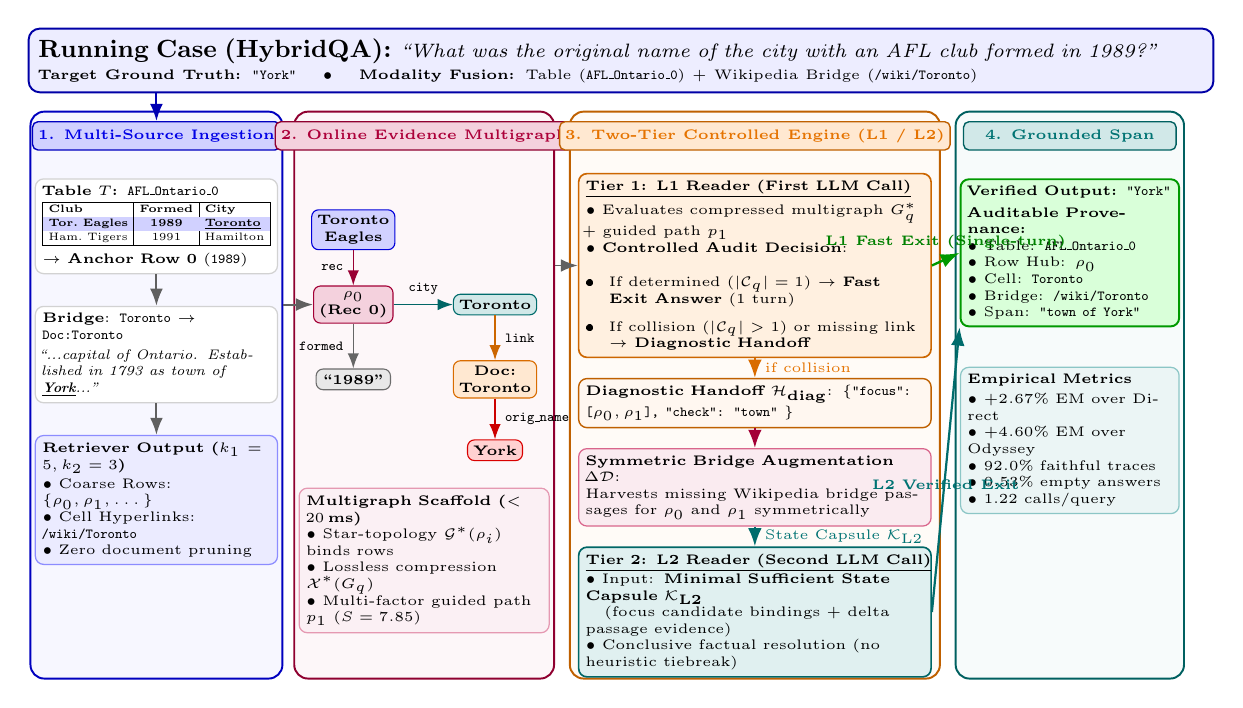
\begin{tikzpicture}[
  >=Latex,
  font=\scriptsize,
  panel/.style={draw=#1!75!black, fill=#1!3, rounded corners=5pt, line width=0.7pt},
  titlebar/.style={fill=#1!18, draw=#1!75!black, line width=0.5pt, rounded corners=2pt, font=\bfseries\tiny, text=#1!90!black, align=center, inner sep=2pt, minimum height=3.6mm},
  subcard/.style={draw=gray!35, fill=white, rounded corners=3pt, align=left, inner sep=2.5pt, font=\tiny, line width=0.45pt},
  llmcard/.style={draw=#1!80!black, fill=#1!12, rounded corners=3pt, align=left, inner sep=2.5pt, font=\tiny, line width=0.6pt},
  flow/.style={->, line width=0.7pt, draw=gray!75!black},
  flow_teal/.style={->, line width=0.8pt, draw=teal!85!black},
  flow_green/.style={->, line width=0.85pt, draw=green!60!black},
  flow_orange/.style={->, line width=0.8pt, draw=orange!85!black},
  flow_purple/.style={->, line width=0.8pt, draw=purple!85!black},
  knode/.style={draw=#1!85!black, fill=#1!18, rounded corners=2.5pt, inner sep=2pt, font=\tiny\bfseries, align=center},
  kedge/.style={->, line width=0.55pt, draw=#1!80!black, font=\tiny}
]

% ========================================================
% TOP BANNER: RUNNING USE CASE QUESTION
% ========================================================
\node[draw=blue!65!black, fill=blue!7, rounded corners=4pt, line width=0.7pt, text width=14.8cm, inner sep=3.5pt, align=left] (q_box) at (7.5, 3.85) {
  \textbf{\small Running Case (HybridQA):} \textit{``What was the original name of the city with an AFL club formed in 1989?''} \\
  \tiny \textbf{Target Ground Truth:} \texttt{"York"} \quad $\bullet$ \quad \textbf{Modality Fusion:} Table (\texttt{AFL\_Ontario\_0}) $+$ Wikipedia Bridge (\texttt{/wiki/Toronto})
};

% ========================================================
% STAGE 1: MULTI-SOURCE INGESTION (BLUE)
% ========================================================
\node[panel=blue, minimum width=3.2cm, minimum height=7.2cm] (panel1) at (1.6, -0.4) {};
\node[titlebar=blue, minimum width=3.0cm] (t1) at ([yshift=-3.2mm]panel1.north) {1. Multi-Source Ingestion};

\node[subcard, text width=2.9cm, anchor=north] (table_box) at ([yshift=-3.5mm]t1.south) {
  {\fontsize{5pt}{6pt}\selectfont
  \textbf{Table $T$: \texttt{AFL\_Ontario\_0}} \\[0.5mm]
  \resizebox{\linewidth}{!}{%
  \renewcommand{\arraystretch}{1.05}%
  \setlength{\tabcolsep}{2.5pt}%
  \begin{tabular}{|l|c|l|}
    \hline
    \textbf{Club} & \textbf{Formed} & \textbf{City} \\
    \hline
    \rowcolor{blue!18} \textbf{Tor.\ Eagles} & \textbf{1989} & \textbf{\underline{Toronto}} \\
    Ham.\ Tigers & 1991 & Hamilton \\
    \hline
  \end{tabular}%
  }\\[0.6mm]
  $\rightarrow$ \textbf{Anchor Row 0} (\texttt{1989})
  \par}
};

\node[subcard, text width=2.9cm, anchor=north] (link_box) at ([yshift=-4mm]table_box.south) {
  {\fontsize{5pt}{6pt}\selectfont
  \textbf{Bridge}: \texttt{Toronto} $\rightarrow$ \texttt{Doc:Toronto} \\[0.4mm]
  \textit{``...capital of Ontario. Established in 1793 as town of \textbf{\underline{York}}...''}
  \par}
};

\node[subcard, text width=2.9cm, fill=blue!8, draw=blue!45, anchor=north] (retr_summary) at ([yshift=-4mm]link_box.south) {
  {\fontsize{5pt}{6pt}\selectfont
  \textbf{Retriever Output ($k_1=5, k_2=3$)} \\[0.3mm]
  $\bullet$ Coarse Rows: $\{\rho_0, \rho_1, \dots\}$ \\
  $\bullet$ Cell Hyperlinks: \texttt{/wiki/Toronto} \\
  $\bullet$ Zero document pruning
  \par}
};

\draw[flow] (table_box.south) -- (link_box.north);
\draw[flow] (link_box.south) -- (retr_summary.north);

% ========================================================
% STAGE 2: SCHEMA-PRESERVING MULTIGRAPH (PURPLE)
% ========================================================
\node[panel=purple, minimum width=3.3cm, minimum height=7.2cm] (panel2) at (5.0, -0.4) {};
\node[titlebar=purple, minimum width=3.1cm] (t2) at ([yshift=-3.2mm]panel2.north) {2. Online Evidence Multigraph};

% Graph nodes
\node[knode=blue] (ent_club) at (4.1, 1.7) {Toronto\\Eagles};
\node[knode=purple] (rec_node) at (4.1, 0.75) {$\rho_0$\\(Rec 0)};
\node[knode=teal] (ent_city) at (5.9, 0.75) {Toronto};
\node[knode=gray] (lit_year) at (4.1, -0.2) {``1989''};
\node[knode=orange] (doc_node) at (5.9, -0.2) {Doc:\\Toronto};
\node[knode=red] (ans_node_g) at (5.9, -1.1) {York};

% Graph edges
\draw[kedge=purple] (ent_club) -- node[left, font=\tiny] {\texttt{rec}} (rec_node);
\draw[kedge=teal] (rec_node) -- node[above, font=\tiny] {\texttt{city}} (ent_city);
\draw[kedge=gray] (rec_node) -- node[left, font=\tiny] {\texttt{formed}} (lit_year);
\draw[kedge=orange] (ent_city) -- node[right, font=\tiny] {\texttt{link}} (doc_node);
\draw[kedge=red] (doc_node) -- node[right, font=\tiny] {\texttt{orig\_name}} (ans_node_g);

\node[subcard, text width=3.0cm, fill=purple!6, draw=purple!40] (graph_props) at (5.0, -2.5) {
  \textbf{Multigraph Scaffold ($<20$\,ms)} \\
  $\bullet$ Star-topology $\mathcal{G}^*(\rho_i)$ binds rows \\
  $\bullet$ Lossless compression $\mathcal{X}^*(G_q)$ \\
  $\bullet$ Multi-factor guided path $p_1$ ($S=7.85$)
};

% ========================================================
% STAGE 3: TWO-TIER CONTROLLED REASONING ENGINE (ORANGE/TEAL)
% ========================================================
\node[panel=orange, minimum width=4.7cm, minimum height=7.2cm] (panel3) at (9.2, -0.4) {};
\node[titlebar=orange, minimum width=4.5cm] (t3) at ([yshift=-3.2mm]panel3.north) {3. Two-Tier Controlled Engine (L1 / L2)};

% L1 LLM Card
\node[llmcard=orange, text width=4.3cm, anchor=north] (l1_box) at ([yshift=-2.8mm]t3.south) {
  {\fontsize{5pt}{6pt}\selectfont
  \textbf{\underline{Tier 1: L1 Reader (First LLM Call)}} \\[0.3mm]
  $\bullet$ Evaluates compressed multigraph $G_q^*$ $+$ guided path $p_1$ \\
  $\bullet$ \textbf{Controlled Audit Decision}:
  \vspace{-0.5mm}
  \begin{itemize}[leftmargin=3mm]
    \setlength{\itemsep}{0pt}
    \item If determined ($|\mathcal{C}_q|=1$) $\rightarrow$ \textbf{Fast Exit Answer} (1 turn)
    \item If collision ($|\mathcal{C}_q|>1$) or missing link $\rightarrow$ \textbf{Diagnostic Handoff}
  \end{itemize}
  \par}
};

% Diagnostic Packet Box
\node[subcard, text width=4.3cm, fill=orange!6, draw=orange!75!black, line width=0.5pt, anchor=north] (handoff_box) at ([yshift=-2.5mm]l1_box.south) {
  {\fontsize{5pt}{6pt}\selectfont
  \textbf{Diagnostic Handoff $\mathcal{H}_{\text{diag}}$}: \texttt{\{"focus": [$\rho_0, \rho_1$], "check": "town" \}}
  \par}
};

% Targeted Bridge Re-retrieval
\node[subcard, text width=4.3cm, fill=purple!8, draw=purple!60, anchor=north] (ret_box) at ([yshift=-2.5mm]handoff_box.south) {
  {\fontsize{5pt}{6pt}\selectfont
  \textbf{Symmetric Bridge Augmentation $\Delta \mathcal{D}$}: \\
  Harvests missing Wikipedia bridge passages for $\rho_0$ and $\rho_1$ symmetrically
  \par}
};

% L2 LLM Card
\node[llmcard=teal, text width=4.3cm, anchor=north] (l2_box) at ([yshift=-2.5mm]ret_box.south) {
  {\fontsize{5pt}{6pt}\selectfont
  \textbf{\underline{Tier 2: L2 Reader (Second LLM Call)}} \\[0.3mm]
  $\bullet$ Input: \textbf{Minimal Sufficient State Capsule $\mathcal{K}_{\text{L2}}$} \\
  \quad (focus candidate bindings $+$ delta passage evidence) \\
  $\bullet$ Conclusive factual resolution (no heuristic tiebreak)
  \par}
};

\draw[flow_orange] (l1_box.south) -- node[right, font=\tiny, text=orange!90!black] {if collision} (handoff_box.north);
\draw[flow_purple] (handoff_box.south) -- (ret_box.north);
\draw[flow_teal] (ret_box.south) -- node[right, font=\tiny, text=teal!90!black] {State Capsule $\mathcal{K}_{\text{L2}}$} (l2_box.north);

% ========================================================
% STAGE 4: GROUNDED ANSWER & PROVENANCE (GREEN)
% ========================================================
\node[panel=teal, minimum width=2.9cm, minimum height=7.2cm] (panel4) at (13.2, -0.4) {};
\node[titlebar=teal, minimum width=2.7cm] (t4) at ([yshift=-3.2mm]panel4.north) {4. Grounded Span};

\node[subcard, text width=2.6cm, fill=green!15, draw=green!60!black, line width=0.7pt, anchor=north] (ans_box) at ([yshift=-3.5mm]t4.south) {
  \textbf{Verified Output: \texttt{"York"}} \\[0.6mm]
  \textbf{Auditable Provenance:} \\
  $\bullet$ Table: \texttt{AFL\_Ontario\_0} \\
  $\bullet$ Row Hub: $\rho_0$ \\
  $\bullet$ Cell: \texttt{Toronto} \\
  $\bullet$ Bridge: \texttt{/wiki/Toronto} \\
  $\bullet$ Span: \texttt{"town of York"}
};

\node[subcard, text width=2.6cm, fill=teal!8, draw=teal!45, anchor=north] (prop_box) at ([yshift=-5mm]ans_box.south) {
  \textbf{Empirical Metrics} \\[0.4mm]
  $\bullet$ $+2.67\%$ EM over Direct \\
  $\bullet$ $+4.60\%$ EM over Odyssey \\
  $\bullet$ $92.0\%$ faithful traces \\
  $\bullet$ $0.53\%$ empty answers \\
  $\bullet$ 1.22 calls/query
};

% ========================================================
% INTER-STAGE CONNECTORS (Two execution branches clearly shown)
% ========================================================
\draw[flow] (panel1.east |- rec_node.west) -- (rec_node.west);
\draw[flow] (panel2.east |- l1_box.west) -- (l1_box.west);

% Branch 1: L1 Fast Exit (Green, upper bypass)
\draw[flow_green] (l1_box.east) -- node[above, font=\tiny\bfseries, text=green!50!black] {L1 Fast Exit (Single-turn)} (ans_box.west);

% Branch 2: L2 Conclusive Resolution (Teal, lower exit)
\draw[flow_teal] (l2_box.east) -- node[below, font=\tiny\bfseries, text=teal!90!black] {L2 Verified Exit} (ans_box.south west);

% Connect top question box
\draw[flow, draw=blue!70!black] (q_box.south -| t1.north) -- (t1.north);

\end{tikzpicture}}
\Description{End-to-end architecture of QEG-RAG illustrating the four stages: Multi-Source Evidence Ingestion, Schema-Preserving Multigraph Construction, Two-Tier Controlled Reasoning Engine, and Grounded Provenance Audit.}
\vspace{2.5mm}
\caption{End-to-end architecture of QEG-RAG. (Sec.~\ref{sec:method-retrieval}) Multi-Source Evidence Ingestion retrieves relevant table rows and linked passages. (Sec.~\ref{sec:method-kg}) Schema-Preserving Multigraph Construction builds star record hubs and text relations without LLMs. (Sec.~\ref{sec:method-engine}) Two-Tier Controlled Reasoning Engine: Tier~1 reads the compressed graph guided by the top reasoning path; clear cases exit immediately in one call, while ambiguous collisions trigger a diagnostic handoff and targeted bridge retrieval for conclusive resolution in Tier~2. (Sec.~\ref{sec:method-answer}) Grounded Generation and Provenance Audit outputs verified spans with full attribution traces.}
\vspace{-2mm}
\label{fig:pipeline}
\end{figure}


To systematically resolve these challenges, QEG-RAG orchestrates four cohesive stages: Stage~1 ingests multimodal evidence; Stage~2 constructs an LLM-free schema-preserving multigraph enforcing tabular semantics ($\rho_i$); Stage~3 scaffolds reasoning paths ($S(p)$) and executes diagnostic-driven retrieval feedback over a bounded two-tier execution protocol ($\mathcal{K}_2$); and Stage~4 conducts grounded generation with provenance auditing.

\paragraph{Problem Formulation and Graph Representation.}
\label{sec:formulation}
We formulate the task of multi-hop question answering over heterogeneous tabular and textual knowledge sources. An input instance is defined as a tuple $\mathcal{I} = (q, T, \mathcal{D}_T)$, where $q$ is a natural language question; $T = (C, R)$ is a semi-structured table comprising ordered headers $C = (c_1, \dots, c_m)$ and rows $R = \{r_1, \dots, r_n\}$ with discrete cells $v_{i,j}$; and $\mathcal{D}_T = \{d_1, \dots, d_K\}$ is the corpus of external text passages associated with $T$, where cell entities connect to external passages via relational mappings $\ell(v_{i,j}) \rightarrow d_k$. The objective is to extract the grounded answer span $a^* \in \mathcal{A}$ along with an auditable reasoning path $p^*$, where $a^*$ may reside as a table cell ($a^* = v_{i,j}$) or as an unstructured text span within a linked passage ($a^* \subset d_k$).

\paragraph{Online Evidence Multigraph Representation.}
Unlike persistent knowledge base settings that depend on static global entity graphs, table--text RAG requires synthesizing unstructured text with tabular structures on-the-fly. For each query $q$, we dynamically instantiate a bounded, query-specific directed multigraph $G_q = (V_q, E_q, \psi_V, \psi_E)$ whose node and edge sets are partitioned as:
\begin{equation}
\label{eq:graph-partition}
V_q = V_{\text{ent}} \cup V_{\text{rec}} \cup V_{\text{lit}}, \qquad
E_q = E_{\text{rec}} \cup E_{\text{attr}} \cup E_{\text{link}} \cup E_{\text{text}}.
\end{equation}
The node partition divides vertices by semantic abstraction:
\begin{itemize}[leftmargin=1.5em]
    \item $V_{\text{ent}}$: Named entity mentions extracted from linked table cells or passage text spans.
    \item $V_{\text{rec}} = \{\rho_i \mid r_i \in R\}$: Local star-topology record hub centroids, where each node $\rho_i = \texttt{table:}T\texttt{:row:}i$ uniquely anchors and binds all cell attributes of row $r_i$ to prevent cross-row attribute conflation.
    \item $V_{\text{lit}}$: Unlinked literal values (e.g., numbers, scores, dates, unlinked strings).
\end{itemize}
The edge set $E_q$ consists of directed relational facts $e = (h, r, t, \pi)$, where $h, t \in V_q$, $r$ is a normalized predicate, and $\pi = (\text{src\_id}, \text{row\_idx}, \text{col\_name})$ stores source provenance:
\begin{itemize}[leftmargin=1.5em]
    \item $E_{\text{rec}} = \{ (u_i, \texttt{has\_record}, \rho_i) \}$: Structural edges connecting row subject entity $u_i$ to its centroid hub $\rho_i$.
    \item $E_{\text{attr}} = \{ (\rho_i, \operatorname{norm}(H_j), v_{i,j}) \}$: Schema-level attribute edges from centroid $\rho_i$ to column cell values $v_{i,j}$.
    \item $E_{\text{link}} = \{ (v_{i,j}, \texttt{linked\_passage}, d_k) \}$: Cross-modal linking edges connecting candidate cells to associated external text passages.
    \item $E_{\text{text}}$: Intra-passage relational triples extracted from retrieved passage sentences.
\end{itemize}

\paragraph{Schema-Preservation and Non-Conflation Property.}
We define the intra-row star subgraph $\mathcal{G}^*(\rho_i) \subset G_q$ for row $r_i$ as:
\begin{equation}
\label{eq:star-subgraph}
\begin{aligned}
\mathcal{G}^*(\rho_i) = \Big( &\{\rho_i, u_i\} \cup \{v_{i,j}\}_{j=1}^m, \\
&\{(u_i, \texttt{has\_record}, \rho_i)\} \cup \{(\rho_i, \operatorname{norm}(H_j), v_{i,j})\}_{j=1}^m \Big).
\end{aligned}
\end{equation}
By construction, for any distinct table rows $r_i, r_{i'} \in R$ ($i \neq i'$), their star centroids are strictly disjoint: $V(\mathcal{G}^*(\rho_i)) \cap V(\mathcal{G}^*(\rho_{i'})) \cap V_{\text{rec}} = \emptyset$. Consequently, every cell value $v_{i,j}$ maintains a unique 1-hop path to its parent record centroid $\rho_i$, structurally preventing horizontal cross-row attribute conflation across symmetric candidate rows without requiring destructive graph pruning.

Once question answering concludes, the dynamic multigraph $G_q$ is discarded, incurring zero persistent graph database index overhead. Throughout this section, we illustrate QEG-RAG via the running HybridQA example depicted in Fig.~\ref{fig:pipeline}: \textit{``What was the original name of the city with an AFL club formed in 1989?''} (ground truth: \texttt{York}).

\subsection{Stage 1: Multi-Source Evidence Ingestion}
\label{sec:method-retrieval}
Given an input table and an associated corpus of external text passages, retrieval operates dynamically at query time:
\begin{itemize}[leftmargin=1.5em]
    \item \emph{Coarse row retrieval and query anchoring}: A lexical retriever indexes table rows with respect to question $q$. A deterministic query anchor inspects $q$ for ordinal constraints (e.g., ``second'', ``last'') and exact schema constraints (column header mentions, numerical filters), selecting top-$k_1$ rows. In Fig.~\ref{fig:pipeline}, the constraint ``formed in 1989'' anchors Row~0 (\texttt{Tor. Eagles}).
    \item \emph{Passage expansion via cross-modal linking}: Rather than retrieving entire document corpora indiscriminately, the passage expander resolves relevant external text passages linked to candidate entities in the top-$k_1$ retrieved rows (via hyperlinks or entity linking) up to a budget of $k_2$ passages. In Fig.~\ref{fig:pipeline}, the bridge cell \texttt{Toronto} in Row~0 links to \texttt{Doc:Toronto}.
\end{itemize}

\subsection{Stage 2: Schema-Preserving Multigraph Construction}
\label{sec:method-kg}
Using the retrieved rows and passages, the system dynamically instantiates the multigraph $G_q=(V_q, E_q)$ without LLM calls:
\begin{itemize}[leftmargin=1.5em]
    \item \emph{Centroid bindings}: For each candidate row $i$, local record centroid $\rho_i \in V_{\text{rec}}$ binds row attributes via $E_{\text{rec}}$ and $E_{\text{attr}}$ (Eq.~\ref{eq:star-subgraph}).
    \item \emph{Cross-modal bridging and text relation extraction}: Edges $E_{\text{link}}$ connect table cell entities to external passage nodes (e.g., $\text{Toronto} \to \text{Doc:Toronto}$). Rule-based text triples $E_{\text{text}}$ link entities to textual attributes (e.g., $\text{Doc:Toronto} \to \text{York}$) deterministically without LLM calls.
\end{itemize}

\subsection{Stage 3: Two-Tier Controlled Reasoning Engine}
\label{sec:method-engine}

\begin{figure}[t]
\centering
\resizebox{\linewidth}{!}{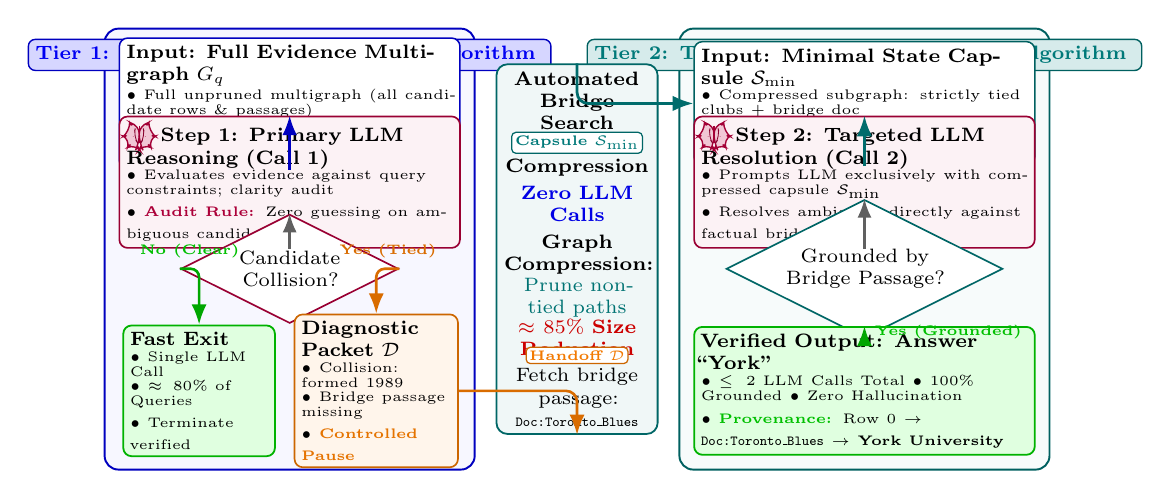
\begin{tikzpicture}[
  >=Latex,
  font=\sffamily\scriptsize,
  % Panels
  col_panel/.style={draw=#1!75!black, fill=#1!3!white, rounded corners=5pt, line width=0.7pt},
  col_hdr/.style={fill=#1!16, draw=#1!75!black, line width=0.5pt, rounded corners=2.5pt, font=\bfseries\scriptsize, text=#1!95!black, inner sep=2.5pt, align=center},
  % Cards matching draw.io
  card_white/.style={draw=#1!75!black, fill=white, rounded corners=3pt, line width=0.55pt, inner sep=2.5pt, align=left, font=\scriptsize},
  card_purple/.style={draw=purple!80!black, fill=purple!5, rounded corners=3pt, line width=0.6pt, inner sep=2.5pt, align=left, font=\scriptsize},
  card_green/.style={draw=green!70!black, fill=green!12, rounded corners=3pt, line width=0.65pt, inner sep=2.5pt, align=left, font=\scriptsize},
  card_orange/.style={draw=orange!80!black, fill=orange!8, rounded corners=3pt, line width=0.6pt, inner sep=2.5pt, align=left, font=\scriptsize},
  card_bridge/.style={draw=teal!80!black, fill=teal!6, rounded corners=4pt, line width=0.65pt, inner sep=2.8pt, align=center, font=\scriptsize},
  % Rhombus Decision
  rhombus_dec/.style={diamond, aspect=2.0, draw=#1!80!black, fill=white, line width=0.6pt, inner sep=1.0pt, align=center, font=\scriptsize},
  % Tags on arrows
  wire_tag/.style={fill=white, draw=#1!80!black, line width=0.45pt, rounded corners=1.5pt, inner sep=1.2pt, font=\bfseries\fontsize{4.6pt}{5.4pt}\selectfont, text=#1!95!black},
  % Arrows
  arr/.style={->, line width=0.85pt, draw=gray!75!black},
  arr_blue/.style={->, line width=0.9pt, draw=blue!75!black},
  arr_green/.style={->, line width=0.95pt, draw=green!65!black},
  arr_orange/.style={->, line width=0.95pt, draw=orange!85!black},
  arr_teal/.style={->, line width=1.0pt, draw=teal!85!black}
]

% Brain icon pic
\tikzset{
  brain_icon/.pic={
    \begin{scope}[scale=0.17]
      \draw[fill=purple!22, draw=purple!85!black, line width=0.5pt]
        (0, 0.72) 
        .. controls (-0.35, 0.82) and (-0.72, 0.62) .. (-0.72, 0.28)
        .. controls (-0.92, 0.12) and (-0.92, -0.22) .. (-0.68, -0.34)
        .. controls (-0.76, -0.58) and (-0.52, -0.78) .. (-0.28, -0.68)
        .. controls (-0.18, -0.82) and (-0.05, -0.68) .. (0, -0.58)
        -- cycle;
      \draw[fill=purple!22, draw=purple!85!black, line width=0.5pt]
        (0, 0.72) 
        .. controls (0.35, 0.82) and (0.72, 0.62) .. (0.72, 0.28)
        .. controls (0.92, 0.12) and (0.92, -0.22) .. (0.68, -0.34)
        .. controls (0.76, -0.58) and (0.52, -0.78) .. (0.28, -0.68)
        .. controls (0.18, -0.82) and (0.05, -0.68) .. (0, -0.58)
        -- cycle;
      \draw[purple!85!black, line width=0.5pt] (0, 0.70) -- (0, -0.56);
      \fill[purple!85!black] (-0.35, 0.3) circle (0.75pt);
      \fill[purple!85!black] (-0.45, -0.1) circle (0.75pt);
      \fill[purple!85!black] (-0.25, -0.4) circle (0.75pt);
      \draw[purple!70!black, line width=0.3pt] (-0.35, 0.3) -- (-0.45, -0.1) -- (-0.25, -0.4);
      \fill[purple!85!black] (0.35, 0.3) circle (0.75pt);
      \fill[purple!85!black] (0.45, -0.1) circle (0.75pt);
      \fill[purple!85!black] (0.25, -0.4) circle (0.75pt);
      \draw[purple!70!black, line width=0.3pt] (0.35, 0.3) -- (0.45, -0.1) -- (0.25, -0.4);
    \end{scope}
  }
}

% =============================================================
% GEOMETRY:
% Width: 12.2 cm
% Col 1: Center X = 2.45cm, Width = 4.7cm (X: 0.10 to 4.80)
% Center: Center X = 6.10cm, Width = 1.9cm (X: 5.15 to 7.05)
% Col 2: Center X = 9.75cm, Width = 4.7cm (X: 7.40 to 12.10)
% Total Height: 5.8 cm (Y: +2.90 to -2.90)
% =============================================================

% -------------------------------------------------------------
% COLUMN 1: TIER 1
% -------------------------------------------------------------
\node[col_panel=blue, minimum width=4.7cm, minimum height=5.6cm] (c1) at (2.45, 0) {};
\node[col_hdr=blue, minimum width=4.4cm, anchor=north] (t1_hdr) at ([yshift=-1.4mm]c1.north) {
  Tier 1: Initial Evidence Reasoning Algorithm
};

% Step 1.1: Input Multigraph
\node[card_white=blue, text width=4.15cm] (t1_in) at (2.45, 1.85) {
  \textbf{Input: Full Evidence Multigraph $G_q$}\\
  {\fontsize{4.6pt}{5.4pt}\selectfont
  $\bullet$ Full unpruned multigraph (all candidate rows \& passages)\\
  $\bullet$ Tied candidates: \texttt{Toronto Eagles} vs \texttt{Toronto Blues} (1989)}
};

% Step 1.2: Primary LLM Reasoning (Call 1)
\node[card_purple, text width=4.15cm] (t1_llm) at (2.45, 0.85) {
  \tikz[baseline=-2.5pt]{\pic {brain_icon};}\hspace{3pt}\textbf{Step 1: Primary LLM Reasoning (Call 1)}\\
  {\fontsize{4.6pt}{5.4pt}\selectfont
  $\bullet$ Evaluates evidence against query constraints; clarity audit\\
  $\bullet$ \textcolor{purple!90!black}{\textbf{Audit Rule:}} Zero guessing on ambiguous candidate ties}
};

% Step 1.3: Rhombus Candidate Collision?
\node[rhombus_dec=purple, text width=1.65cm] (t1_dec) at (2.45, -0.25) {
  Candidate\\Collision?
};

% Step 1.4a: Fast Exit (Branch: No)
\node[card_green, text width=1.75cm] (t1_exit) at (1.30, -1.80) {
  \textbf{Fast Exit}\\[0.2mm]
  {\fontsize{4.5pt}{5.2pt}\selectfont
  $\bullet$ Single LLM Call\\
  $\bullet$ $\approx 80\%$ of Queries\\
  $\bullet$ Terminate verified}
};

% Step 1.4b: Diagnostic Packet D (Branch: Yes)
\node[card_orange, text width=1.90cm] (t1_out) at (3.55, -1.80) {
  \textbf{Diagnostic Packet $\mathcal{D}$}\\[0.2mm]
  {\fontsize{4.5pt}{5.2pt}\selectfont
  $\bullet$ Collision: formed 1989\\
  $\bullet$ Bridge passage missing\\
  $\bullet$ \textcolor{orange!90!black}{\textbf{Controlled Pause}}}
};

% Connectors in Tier 1
\draw[arr_blue] (t1_in) -- (t1_llm);
\draw[arr] (t1_llm) -- (t1_dec);
\draw[arr_green, rounded corners=3pt] (t1_dec.west) -| node[above, font=\bfseries\tiny, text=green!75!black, near start] {No (Clear)} (t1_exit.north);
\draw[arr_orange, rounded corners=3pt] (t1_dec.east) -| node[above, font=\bfseries\tiny, text=orange!85!black, near start] {Yes (Tied)} (t1_out.north);


% -------------------------------------------------------------
% COLUMN 2: TIER 2
% -------------------------------------------------------------
\node[col_panel=teal, minimum width=4.7cm, minimum height=5.6cm] (c2) at (9.75, 0) {};
\node[col_hdr=teal, minimum width=4.4cm, anchor=north] (t2_hdr) at ([yshift=-1.4mm]c2.north) {
  Tier 2: Targeted Collision Resolution Algorithm
};

% Step 2.1: Input Minimal Capsule
\node[card_white=teal, text width=4.15cm] (t2_in) at (9.75, 1.85) {
  \textbf{Input: Minimal State Capsule $\mathcal{S}_{\mathrm{min}}$}\\
  {\fontsize{4.6pt}{5.4pt}\selectfont
  $\bullet$ Compressed subgraph: strictly tied clubs + bridge doc\\
  $\bullet$ Zero non-competing candidates; eliminates context dilution}
};

% Step 2.2: Targeted LLM Call (Call 2)
\node[card_purple, text width=4.15cm] (t2_llm) at (9.75, 0.85) {
  \tikz[baseline=-2.5pt]{\pic {brain_icon};}\hspace{3pt}\textbf{Step 2: Targeted LLM Resolution (Call 2)}\\
  {\fontsize{4.6pt}{5.4pt}\selectfont
  $\bullet$ Prompts LLM exclusively with compressed capsule $\mathcal{S}_{\mathrm{min}}$\\
  $\bullet$ Resolves ambiguity directly against factual bridge evidence}
};

% Step 2.3: Rhombus Grounded by Bridge?
\node[rhombus_dec=teal, text width=2.3cm] (t2_dec) at (9.75, -0.25) {
  Grounded by\\Bridge Passage?
};

% Step 2.4: Verified Output
\node[card_green, text width=4.15cm] (t2_out) at (9.75, -1.80) {
  \textbf{Verified Output: Answer ``York''}\\[0.2mm]
  {\fontsize{4.6pt}{5.4pt}\selectfont
  $\bullet$ $\le 2$ LLM Calls Total $\bullet$ 100\% Grounded $\bullet$ Zero Hallucination\\
  $\bullet$ \textcolor{green!75!black}{\textbf{Provenance:}} Row 0 $\to$ \texttt{Doc:Toronto\_Blues} $\to$ \textbf{York University}}
};

% Connectors in Tier 2
\draw[arr_teal] (t2_in) -- (t2_llm);
\draw[arr] (t2_llm) -- (t2_dec);
\draw[arr_green] (t2_dec.south) -- node[right, font=\bfseries\tiny, text=green!75!black] {Yes (Grounded)} (t2_out.north);


% -------------------------------------------------------------
% CENTER: BRIDGE SEARCH & GRAPH COMPRESSION
% -------------------------------------------------------------
\node[card_bridge, text width=1.85cm] (bridge) at (6.10, 0.00) {
  \textbf{Automated Bridge Search}\\[-0.2mm]
  \textbf{\& Graph Compression}\\[0.6mm]
  \textcolor{blue!90!black}{\textbf{Zero LLM Calls}}\\[0.6mm]
  \textbf{Graph Compression:}\\[-0.2mm]
  \textcolor{teal!90!black}{Prune non-tied paths}\\[-0.2mm]
  \textcolor{red!80!black}{\textbf{$\approx 85\%$ Size Reduction}}\\[0.5mm]
  Fetch bridge passage:\\
  {\fontsize{4.2pt}{5.0pt}\selectfont \texttt{Doc:Toronto\_Blues}}
};

% Inter-tier connecting wires
\draw[arr_orange, rounded corners=4pt] (t1_out.east) -- (6.10, -1.80) -- (bridge.south);
\draw[arr_teal, rounded corners=4pt] (bridge.north) -- (6.10, 1.85) -- (t2_in.west);

% Clean wire tags
\node[wire_tag=orange] at (6.10, -1.35) {Handoff $\mathcal{D}$};
\node[wire_tag=teal] at (6.10, 1.35) {Capsule $\mathcal{S}_{\mathrm{min}}$};

\end{tikzpicture}
}
\vspace{2mm}
\caption{Architecture of the bounded two-tier controlled reasoning engine. (Top) Tier~1 evaluates the complete unpruned evidence graph under guided path scaffolding. When the evidence is clear and unambiguous, execution terminates immediately via Fast Exit in a single LLM call ($\approx 80\%$ of queries). When ambiguity or a missing bridge link occurs, the model emits a structured diagnostic handoff. (Bottom) An automated search fetches targeted bridge evidence for the competing candidates to form a minimal focused state capsule. Tier~2 resolves the ambiguity by verified factual evidence in a second call, strictly bounding total execution to at most two calls.}
\vspace{-2mm}
\label{fig:two-tier}
\end{figure}


QEG-RAG resolves the operational dilemma between destructive graph pruning and unbounded agentic loops. As depicted in the end-to-end pipeline (Fig.~\ref{fig:pipeline}, Stage~3) and detailed in Fig.~\ref{fig:two-tier}, the reasoning engine decouples execution into two strictly bounded tiers connected by an automated diagnostic bridge:

\paragraph{Tier 1: Primary Reader (First Call).}
Tier~1 evaluates the initial multimodal evidence without destructive pruning. To prevent token overflow while retaining complete context, the multigraph $G_q$ is serialized into compact record blocks and deduplicated passage texts:
\begin{equation}
\label{eq:compression}
\mathcal{X}^*(G_q) = \operatorname{Enc}_{\text{table}}\left(\{\mathcal{G}^*(\rho_i)\}_{i=1}^{k_1}\right) \;\parallel\; \operatorname{Enc}_{\text{text}}(\mathcal{D}_{\text{unique}}),
\end{equation}
where $\mathcal{D}_{\text{unique}}$ indexes each external passage once by source identifier, eliminating redundant text while preserving complete evidence facts. Alongside the unpruned graph, candidate reasoning paths $p = (v_0, e_1, \dots, e_L, v_L)$ are scored via a multi-factor linear objective:
\begin{equation}
\label{eq:path-score}
S(p) = \mathbf{w}^\top \boldsymbol{\phi}(p, q) - \lambda \cdot |p|,
\end{equation}
where $\boldsymbol{\phi}(p, q)$ captures question entity overlap, table--text transitions, row consistency, and entity support, while $\lambda \cdot |p|$ penalizes redundant hops. The top-scoring path $p_1 = \arg\max_{p} S(p)$ serves as a non-filtering reading scaffold that steers model attention along verified cross-modal relations.

The language model $\mathcal{M}$ evaluates the primary context $\mathcal{X}_1 = (q, \mathcal{X}^*(G_q), p_1)$. Let $\mathcal{C}_q$ denote the set of candidate record centroids supported by top-scoring paths. The model executes an adaptive audit decision:
\begin{enumerate}
    \item \emph{Fast Exit}: If candidate evidence is unambiguous ($|\mathcal{C}_q| = 1$) and the reasoning path is intact, the model outputs the verified answer span directly:
    \begin{equation}
    a^* = \arg\max_{a \in \mathcal{A}} P_{\mathcal{M}}(a \mid \mathcal{X}_1),
    \end{equation}
    concluding execution immediately in a single call ($\approx 80\%$ of queries).
    \item \emph{Diagnostic Handoff}: If candidate collisions occur across symmetric rows ($|\mathcal{C}_q| > 1$) or a bridge passage link is missing, the model is strictly prevented from ungrounded guessing. Instead, it emits a structured diagnostic packet:
    \begin{equation}
    \mathcal{H}_{\text{diag}} = \big(\mathcal{C}_{\text{focus}}, \, \beta, \, \psi_{\text{check}}\big),
    \end{equation}
    where $\mathcal{C}_{\text{focus}}$ designates the competing candidate rows, $\beta$ identifies the blocker type (candidate collision or missing bridge), and $\psi_{\text{check}}$ specifies the unresolved factual predicate.
\end{enumerate}

\paragraph{Diagnostic Handoff and Targeted Bridge Augmentation.}
Upon receiving $\mathcal{H}_{\text{diag}}$, an automated retriever (0 LLM calls) fetches missing candidate bridge passages $\Delta\mathcal{D}$ exclusively for the disputed candidate rows $\mathcal{C}_{\text{focus}}$:
\begin{equation}
\label{eq:targeted-retrieval}
\Delta \mathcal{D} = \bigcup_{c \in \mathcal{C}_{\text{focus}}} \left( \ell(c) \setminus \mathcal{D}_{\text{current}} \right),
\end{equation}
enforcing a symmetric per-candidate retrieval quota to maintain evidentiary balance. The targeted evidence is packaged into a minimal sufficient state capsule $\mathcal{K}_2$:
\begin{equation}
\label{eq:l2-capsule}
\mathcal{K}_2 = \left( q, \, \psi_{\text{check}}, \, \{ \mathcal{G}^*(\rho_c) \}_{c \in \mathcal{C}_{\text{focus}}}, \, \Delta \mathcal{D} \right).
\end{equation}
Unlike the broad Tier~1 context, $\mathcal{K}_2$ discards unrelated rows and concentrates exclusively on verifying the disputed hypotheses.

\paragraph{Tier 2: Targeted Reader (Second Call).}
In Tier~2, the language model evaluates the focused state capsule $\mathcal{K}_2$ to perform conclusive factual resolution:
\begin{equation}
a^* = \arg\max_{a \in \mathcal{A}} P_{\mathcal{M}}(a \mid \mathcal{K}_2).
\end{equation}
This resolves candidate collisions through verified evidence rather than heuristic tiebreaking, with total inference overhead strictly bounded to at most two calls.

\subsection{Stage 4: Grounded Generation and Provenance Audit}
\label{sec:method-answer}
Stage~4 outputs the verified answer span and exports an inspectable provenance homomorphism $\pi: a^* \rightarrow E_q^*$, mapping the answer back to traversed table coordinates (\texttt{AFL\_Ontario\_0:row:0}), bridge URLs (\texttt{/wiki/Toronto}), and passage text excerpts (\texttt{town of York (1793)}). If graph search disconnects, \emph{reverse grounding} synthesizes directly over retrieved evidence and maps the extracted span back onto $G_q$, avoiding empty failures.

\section{Experimental Protocol}
\label{sec:experiments}

\subsection{Benchmark Datasets and Evaluation Metrics}
We evaluate across two challenging multi-hop table--text benchmarks ($N=1{,}500$ each): (1)~\emph{HybridQA}~\cite{hybridqa}, evaluating multi-hop reasoning over Wikipedia tables aligned with hyperlinked passages; and (2)~\emph{OTT-QA}~\cite{chen2021ottqa}, evaluating open table-and-text retrieval and question answering where candidate tables and text spans must be fetched and grounded jointly. Both benchmark subsets strictly preserve the stratified multimodal reasoning distribution across numeric and textual answer modalities.

\paragraph{Evaluation Scope: Zero-Shot In-Context RAG vs.\ Supervised Fine-Tuning.}
We explicitly clarify the operational scope of this evaluation. While task-specific supervised models (e.g., MuGER$^2$~\cite{chen2022muger2}, S3HQA~\cite{lei2023s3hqa}) achieve higher leaderboard numbers by fine-tuning millions of parameters over the 62k labeled training instances of HybridQA, they are specialized to fixed benchmark distributions and cannot generalize to ad-hoc, out-of-domain tables without expensive re-annotation and re-training. In contrast, QEG-RAG operates in the strictly training-free, zero-shot in-context RAG regime (0 training examples, 0 updated weights). Under this practical setting, our primary comparisons are appropriately framed against published zero-shot hybrid graph frameworks (e.g., ODYSSEY~\cite{agarwal2025hybrid}) and in-context LLM baselines under identical context and retrieval budgets.

\paragraph{Strict Context-Grounded Protocol.}
To rigorously assess faithful reasoning and prevent models from relying on latent parametric memorization (e.g., pre-trained Wikipedia facts), all systems are evaluated under a strict context-grounding protocol. Prompts mandate that answers must be derived exclusively from the provided tabular and textual evidence; when the factual chain is broken or evidence is insufficient, the model must output an ungrounded or empty response rather than guessing. This protocol faithfully mirrors enterprise and scientific environments where hallucination is unacceptable.

We report three standard accuracy metrics: (1)~\emph{Exact Match (EM)} under standard normalization; (2)~\emph{Token-level F1}; and (3)~\emph{Semantic Exact Match (Semantic EM)} tolerating surface aliases. System efficiency is reported via average LLM calls and ungrounded empty answer percentage.

\enlargethispage{3.5\baselineskip}
\subsection{Baselines and Experimental Settings}
Methods are evaluated across two model paradigms under identical retrieval pools ($k_1=5, k_2=3$), context budgets ($24{,}000$ chars), and greedy decoding ($T=0$): (i)~\emph{Native Reasoning}: GPT-OSS 20B and 120B, featuring internal thinking tokens; and (ii)~\emph{Standard Non-Reasoning}: Qwen 122B (\texttt{Qwen2.5-72B/122B-Instruct}), a flagship instruction-tuned LLM without test-time reasoning. We compare five configurations: (1)~\emph{Direct LLM}: Prompting over linearized rows and passages; (2)~\emph{ODYSSEY}~\cite{agarwal2025hybrid}: Zero-shot hybrid graph with destructive pruning; (3)~\emph{Graph w/o Path}: Unpruned multigraph without linear path sequences; (4)~\emph{Path-Text Top-$N$}: Hard filtering to top-$N$ ranked paths; and (5)~\emph{QEG-RAG (Ours)}: Full evidence multigraph with path scaffolding and two-tier diagnostic guidance.

\begin{table}[t]
\vspace{-2mm}
\caption{Comprehensive comparative evaluation of native reasoning models across multi-hop table--text benchmarks under strict context grounding ($k_1=5, k_2=3$, 24k context budget, $N=1{,}500$ per benchmark).}
\label{tab:main-results}
\centering
\scriptsize
\renewcommand{\arraystretch}{0.88}
\resizebox{\textwidth}{!}{%
\begin{tabular}{@{}lllrrrrr@{}}
\toprule
Dataset & Model & Method & EM (\%) & $\text{F}_1$ (\%) & Sem.\ EM & Empty & Calls \\
\midrule
\multirow{10}{*}{HybridQA} & \multirow{5}{*}{GPT-OSS 20B}  
  & Direct LLM               & 45.73 & 54.25 & 48.00 & 30.20\% & \textbf{1.00} \\
& & ODYSSEY~\cite{agarwal2025hybrid} & 32.80 & 39.98 & 34.80 & 41.87\% & 5.39 \\
& & Graph w/o Path           & 31.80 & 37.92 & 32.93 & 46.00\% & \textbf{1.00} \\
& & Path-Text Top-$N$        & 10.87 & 12.53 & 10.93 & 79.13\% & \textbf{1.00} \\
& & \textbf{QEG-RAG (Ours)}  & \textbf{53.07} & \textbf{66.45} & \textbf{54.07} & \textbf{11.53\%} & 1.23 \\
\cmidrule{2-8}
& \multirow{5}{*}{GPT-OSS 120B} 
  & Direct LLM               & 56.20 & 65.62 & 57.87 & 20.00\% & \textbf{1.00} \\
& & ODYSSEY~\cite{agarwal2025hybrid} & 37.80 & 45.17 & 39.13 & 38.87\% & 5.38 \\
& & Graph w/o Path           & 33.93 & 39.80 & 34.67 & 48.07\% & \textbf{1.00} \\
& & Path-Text Top-$N$        & 13.07 & 15.13 & 13.13 & 75.53\% & \textbf{1.00} \\
& & \textbf{QEG-RAG (Ours)}  & \textbf{59.27} & \textbf{70.70} & \textbf{60.00} & \textbf{10.73\%} & 1.20 \\
\midrule
\multirow{10}{*}{OTT-QA}   & \multirow{5}{*}{GPT-OSS 20B}  
  & Direct LLM               & 50.80 & 57.70 & 51.80 & 30.00\% & \textbf{1.00} \\
& & ODYSSEY~\cite{agarwal2025hybrid} & 37.47 & 43.66 & 38.60 & 40.73\% & 5.44 \\
& & Graph w/o Path           & 40.87 & 46.35 & 41.60 & 39.53\% & \textbf{1.00} \\
& & Path-Text Top-$N$        & 9.40  & 10.39 & 9.47  & 82.20\% & \textbf{1.00} \\
& & \textbf{QEG-RAG (Ours)}  & \textbf{55.60} & \textbf{67.59} & \textbf{55.93} & \textbf{11.87\%} & 1.24 \\
\cmidrule{2-8}
& \multirow{5}{*}{GPT-OSS 120B} 
  & Direct LLM               & 60.40 & 67.93 & 61.20 & 21.20\% & \textbf{1.00} \\
& & ODYSSEY~\cite{agarwal2025hybrid} & 41.73 & 47.96 & 42.53 & 39.47\% & 5.48 \\
& & Graph w/o Path           & 42.27 & 47.58 & 42.87 & 40.87\% & \textbf{1.00} \\
& & Path-Text Top-$N$        & 13.20 & 14.88 & 13.27 & 75.93\% & \textbf{1.00} \\
& & \textbf{QEG-RAG (Ours)}  & \textbf{62.93} & \textbf{73.03} & \textbf{63.07} & \textbf{10.80\%} & 1.22 \\
\bottomrule
\end{tabular}%
}
\vspace{-2.5mm}
\end{table}

\section{Results and In-Depth Analysis}
\label{sec:results}

\paragraph{Main Benchmark Results on Native Reasoning Models.}
Table~\ref{tab:main-results} reports performance across both benchmarks ($N=1{,}500$ each) under native reasoning models. QEG-RAG consistently achieves superior grounding accuracy: on HybridQA with GPT-OSS 20B, it reaches 53.07\% EM and 66.45\% $\text{F}_1$ (+7.34\% EM over Direct LLM; +20.27\% over ODYSSEY); on 120B, it achieves 59.27\% EM and 70.70\% $\text{F}_1$ (+3.07\% EM over Direct LLM; +21.47\% over ODYSSEY, McNemar $p < 0.001$). On open retrieval (OTT-QA), QEG-RAG demonstrates identical gains, achieving 55.60\% EM on 20B (+4.80\% over Direct LLM) and 62.93\% EM on 120B (+2.53\% over Direct LLM). In contrast, destructive graph pruning (ODYSSEY) and hard path filtering (Path-Text) collapse across benchmarks, suffering 38\%--82\% ungrounded empty abstentions due to peripheral evidence loss.

\paragraph{Cross-Paradigm Generalization: Overcoming the Over-Abstention Trap.}
While native reasoning models use internal thinking tokens, standard instruction-tuned LLMs lack test-time reasoning. In Table~\ref{tab:qwen-results}, under strict grounding, non-reasoning models (Qwen 122B on OTT-QA) suffer an \emph{over-abstention trap}: Direct LLM emits 65.80\% empty responses, while ODYSSEY surges to 92.07\% empty (5.93\% EM), as disconnected triples prevent token-level resolution. QEG-RAG serves as an \emph{external neuro-symbolic reasoning scaffold}: providing deterministic path sequences and diagnostic bridge evidence, it eliminates empty failures (0.00\% Empty) and elevates EM to 33.40\% (+4.13\% over Direct LLM; $5.6\times$ higher than ODYSSEY), extending robustly to architectures without native reasoning.

\begin{table}[t]
\vspace{-2mm}
\caption{Cross-paradigm generalization on standard non-reasoning instruction-tuned LLM (Qwen 122B on OTT-QA, $N=1{,}500$). QEG-RAG acts as an external neuro-symbolic scaffold, eliminating empty abstentions and elevating EM.}
\label{tab:qwen-results}
\centering
\scriptsize
\renewcommand{\arraystretch}{0.88}
\setlength{\tabcolsep}{5.5pt}
\begin{tabular}{@{}lrrrrr@{}}
\toprule
Method & EM (\%) & $\text{F}_1$ (\%) & Sem.\ EM & Empty & Calls \\
\midrule
Direct LLM                       & 29.27 & 31.52 & 29.53 & 65.80\% & \textbf{1.00} \\
ODYSSEY~\cite{agarwal2025hybrid} & 5.93  & 6.99  & 5.93  & 92.07\% & 6.66 \\
Graph w/o Path                   & 9.93  & 11.00 & 10.00 & 88.47\% & \textbf{1.00} \\
Path-Text Top-$N$                & 1.67  & 1.89  & 1.73  & 97.53\% & \textbf{1.00} \\
\textbf{QEG-RAG (Ours)}          & \textbf{33.40} & \textbf{35.30} & \textbf{33.53} & \textbf{0.00\%} & 1.64 \\
\bottomrule
\end{tabular}
\vspace{-2.5mm}
\end{table}\enlargethispage{3.5\baselineskip}
We structure our empirical analysis around research questions directly investigating our core contributions:

\noindent\emph{RQ1 (Explicit Reasoning Guidance):} \emph{How effectively does deterministic path scaffolding steer LLM attention along multi-hop cross-modal evidence without destructive evidence pruning?} Supplying an unorganized edge set disperses LLM attention. In Table~\ref{tab:ablation} (Row~6), providing the complete multigraph without path sequences retains strong performance (61.60\% EM), demonstrating that QEG's schema-preserving topology alone provides flexible multi-hop reach, while path scaffolding directs focus along verified relations, yielding 92.0\% provenance faithfulness in our human audit.

\noindent\emph{RQ2 (Diagnostic Feedback \& Bounded Efficiency):} \emph{Can QEG-RAG resolve retrieval collisions factually while bounding execution overhead against unbounded agent loops?} (a)~\emph{Destructive pruning causes evidence loss}: Peripheral links severed by ODYSSEY surge empty abstentions (up to 41.87\% on 20B, 92.07\% on Qwen 122B) and depress EM to 5.93\%--37.80\%. Path-Text Top-$N$ hard filtering collapses further (EM 1.67\%--13.07\%). In Table~\ref{tab:ablation} (Row~1), disabling lossless prompt compression causes EM to collapse by $-27.60\%$ with $52.40\%$ empty answers from token blowout. QEG-RAG retains 100\% evidence via lossless compression. (b)~\emph{Diagnostic feedback and bounded efficiency}: Rather than unbounded agent loops (e.g., HydraRAG) or heuristic tiebreaking, QEG-RAG concludes unambiguous queries in a single primary call (Fast Exit), reserving a targeted second call only when diagnostic feedback identifies collisions or missing passages. Omitting targeted Tier-2 evidence (Row~3) or diagnostic focus (Row~4) degrades performance by $-3.20\%$ and $-1.40\%$ EM, while omitting Tier~2 entirely (Row~5) drops F1 by $-7.68\%$ on difficult collisions. QEG-RAG averages only 1.20--1.24 calls per query, achieving high accuracy with strictly bounded latency.

\noindent\emph{RQ3 (Preservation of Tabular Semantics):} \emph{Does the star centroid formulation prevent cross-row attribute conflation under symmetric candidate rows without LLM extraction costs?} In Direct LLM, linearizing tables decouples cell values from originating rows, causing attribute conflation when multiple symmetric rows satisfy partial conditions. Across both paradigms, QEG-RAG achieves higher exact match by anchoring row attributes to column predicates via centroids $\rho_i$, maintaining Row Attribute Non-Conflation. In Table~\ref{tab:ablation} (Row~2), eliminating centroids $\rho_i$ drops EM by $-3.00\%$ and F1 by $-5.32\%$, while nearly doubling empty abstentions from $11.40\%$ to $19.60\%$, validating structural row bindings.

\begin{table}[t]
\vspace{-4mm}
\caption{Systematic knockout ablation study on pooled partitions ($N=500$ under GPT-OSS 120B). All variants isolate individual components against full QEG-RAG.}
\label{tab:ablation}
\centering
\scriptsize
\renewcommand{\arraystretch}{0.82}
\setlength{\tabcolsep}{1.8pt}
\resizebox{\linewidth}{!}{%
\begin{tabular}{@{}lrrrrp{3.75cm}@{}}
\toprule
Ablation Configuration & EM (\%) & F1 (\%) & $\Delta$EM & Empty & Architectural Implication \\
\midrule
\textbf{Full QEG-RAG (Two-Tier)} & \textbf{59.20} & \textbf{68.06} & --- & \textbf{11.40\%} & Full controlled evidence scaffolding \\
\midrule
(1) w/o Prompt Compression       & 31.60 & 37.36 & $-27.60$ & 52.40\% & Token blowout; $>52\%$ empty abstentions \\
(2) w/o Record Nodes $\rho_i$    & 56.20 & 62.74 & $-3.00$  & 19.60\% & Cross-row conflation; doubles empty rate \\
(3) w/o Tier-2 Targeted Evidence & 56.00 & 63.60 & $-3.20$  & 18.40\% & Re-reading misses external bridge facts \\
(4) w/o Diagnostic Focus         & 57.80 & 65.74 & $-1.40$  & 15.60\% & Lack of cell-level grounding harms F1 \\
(5) w/o Adaptive Tier-2 (Single Tier-1) & 58.60 & 66.78 & $-0.60$  & 5.40\%  & Single tier fails on collisions ($-7.68\%$ F1) \\
(6) w/o Path Guidance (Graph)    & 61.60 & 70.14 & $+2.40$  & 11.80\% & Flexible reach via multigraph topology \\
\bottomrule
\end{tabular}%
}
\vspace{-4mm}
\end{table}

\paragraph{Summary of Knockout Ablations \& Provenance Audit.}
Table~\ref{tab:ablation} confirms all architectural pillars are non-redundant. A manual audit on 100 questions confirms: (1)~\emph{Trace Faithfulness}: 92.0\% produce faithful chains to verified evidence; (2)~\emph{Bridge Alignment}: 89.0\% identify ground-truth bridges; and (3)~\emph{Empty Failure Reduction}: on 120B, QEG-RAG reduces empty failures to 0.53\% (vs.\ 3.40\% for ODYSSEY).

\enlargethispage{6.0\baselineskip}
\section{Limitations}
\label{sec:limitations}
While QEG-RAG effectively structures and reasons over retrieved context without destructive pruning, downstream performance remains bounded by the completeness of upstream evidence retrieval. Further advancing evidence search and multi-hop retrieval strategies presents a direct pathway to further elevate Exact Match (EM) accuracy on complex questions.

\section{Conclusion}
\label{sec:conclusion}
We presented QEG-RAG, uniting query-time evidence graphs with path-scaffolded diagnostic reasoning for faithful table--text question answering. By combining schema-preserving multigraphs, compact lossless compression, deterministic path scaffolding, and adaptive two-tier diagnostic verification, QEG-RAG resolves the dilemma between destructive graph pruning and unbounded agent loops. Across both reasoning and non-reasoning paradigms under strict context grounding, QEG-RAG consistently achieves higher grounding accuracy, eliminates empty failures, and provides auditable provenance within a bounded 1-to-2 call budget.

\makeatletter
\renewenvironment{thebibliography}[1]
     {\section*{\refname}%
      \def\@biblabel##1{##1.}%
      \fontsize{6.4pt}{7.4pt}\selectfont
      \list{\@biblabel{\@arabic\c@enumiv}}%
           {\settowidth\labelwidth{\@biblabel{#1}}%
            \leftmargin\labelwidth
            \advance\leftmargin\labelsep
            \setlength{\itemsep}{-0.5pt plus 0.2pt}%
            \setlength{\parsep}{0pt}%
            \setlength{\topsep}{0.6pt}%
            \usecounter{enumiv}%
            \let\p@enumiv\@empty
            \renewcommand\theenumiv{\@arabic\c@enumiv}}%
      \renewcommand\newblock{\hskip .11em \@plus.33em \@minus.07em}%
      \sloppy\clubpenalty4000\widowpenalty4000%
      \sfcode`\.=1000\relax}
     {\def\@noitemerr
       {\@latex@warning{Empty `thebibliography' environment}}%
      \endlist}
\makeatother
\bibliographystyle{splncs04_unsrt}
\bibliography{refs}


\end{document}
